\insertbigimage{figures/block_diagram.pdf}{Block diagram of the system}{block_diagram}

\section{System Design Overview}

The system was designed around the RP2040 microcontroller, acting as the central 
processing unit for interfacing with a variety of sensors and control devices. 
The design incorporates the SF-5M sap flow sensor, LT-1T leaf temperature sensor, 
and MT-603 load cell to measure various environmental parameters. Each of these 
sensors use different communication protocols, requiring careful consideration of 
power requirements, signal integrity, and communication compatibility. \cref{block_diagram} 
shows an overview of all the communication systems involved in the design.

\begin{figure}
    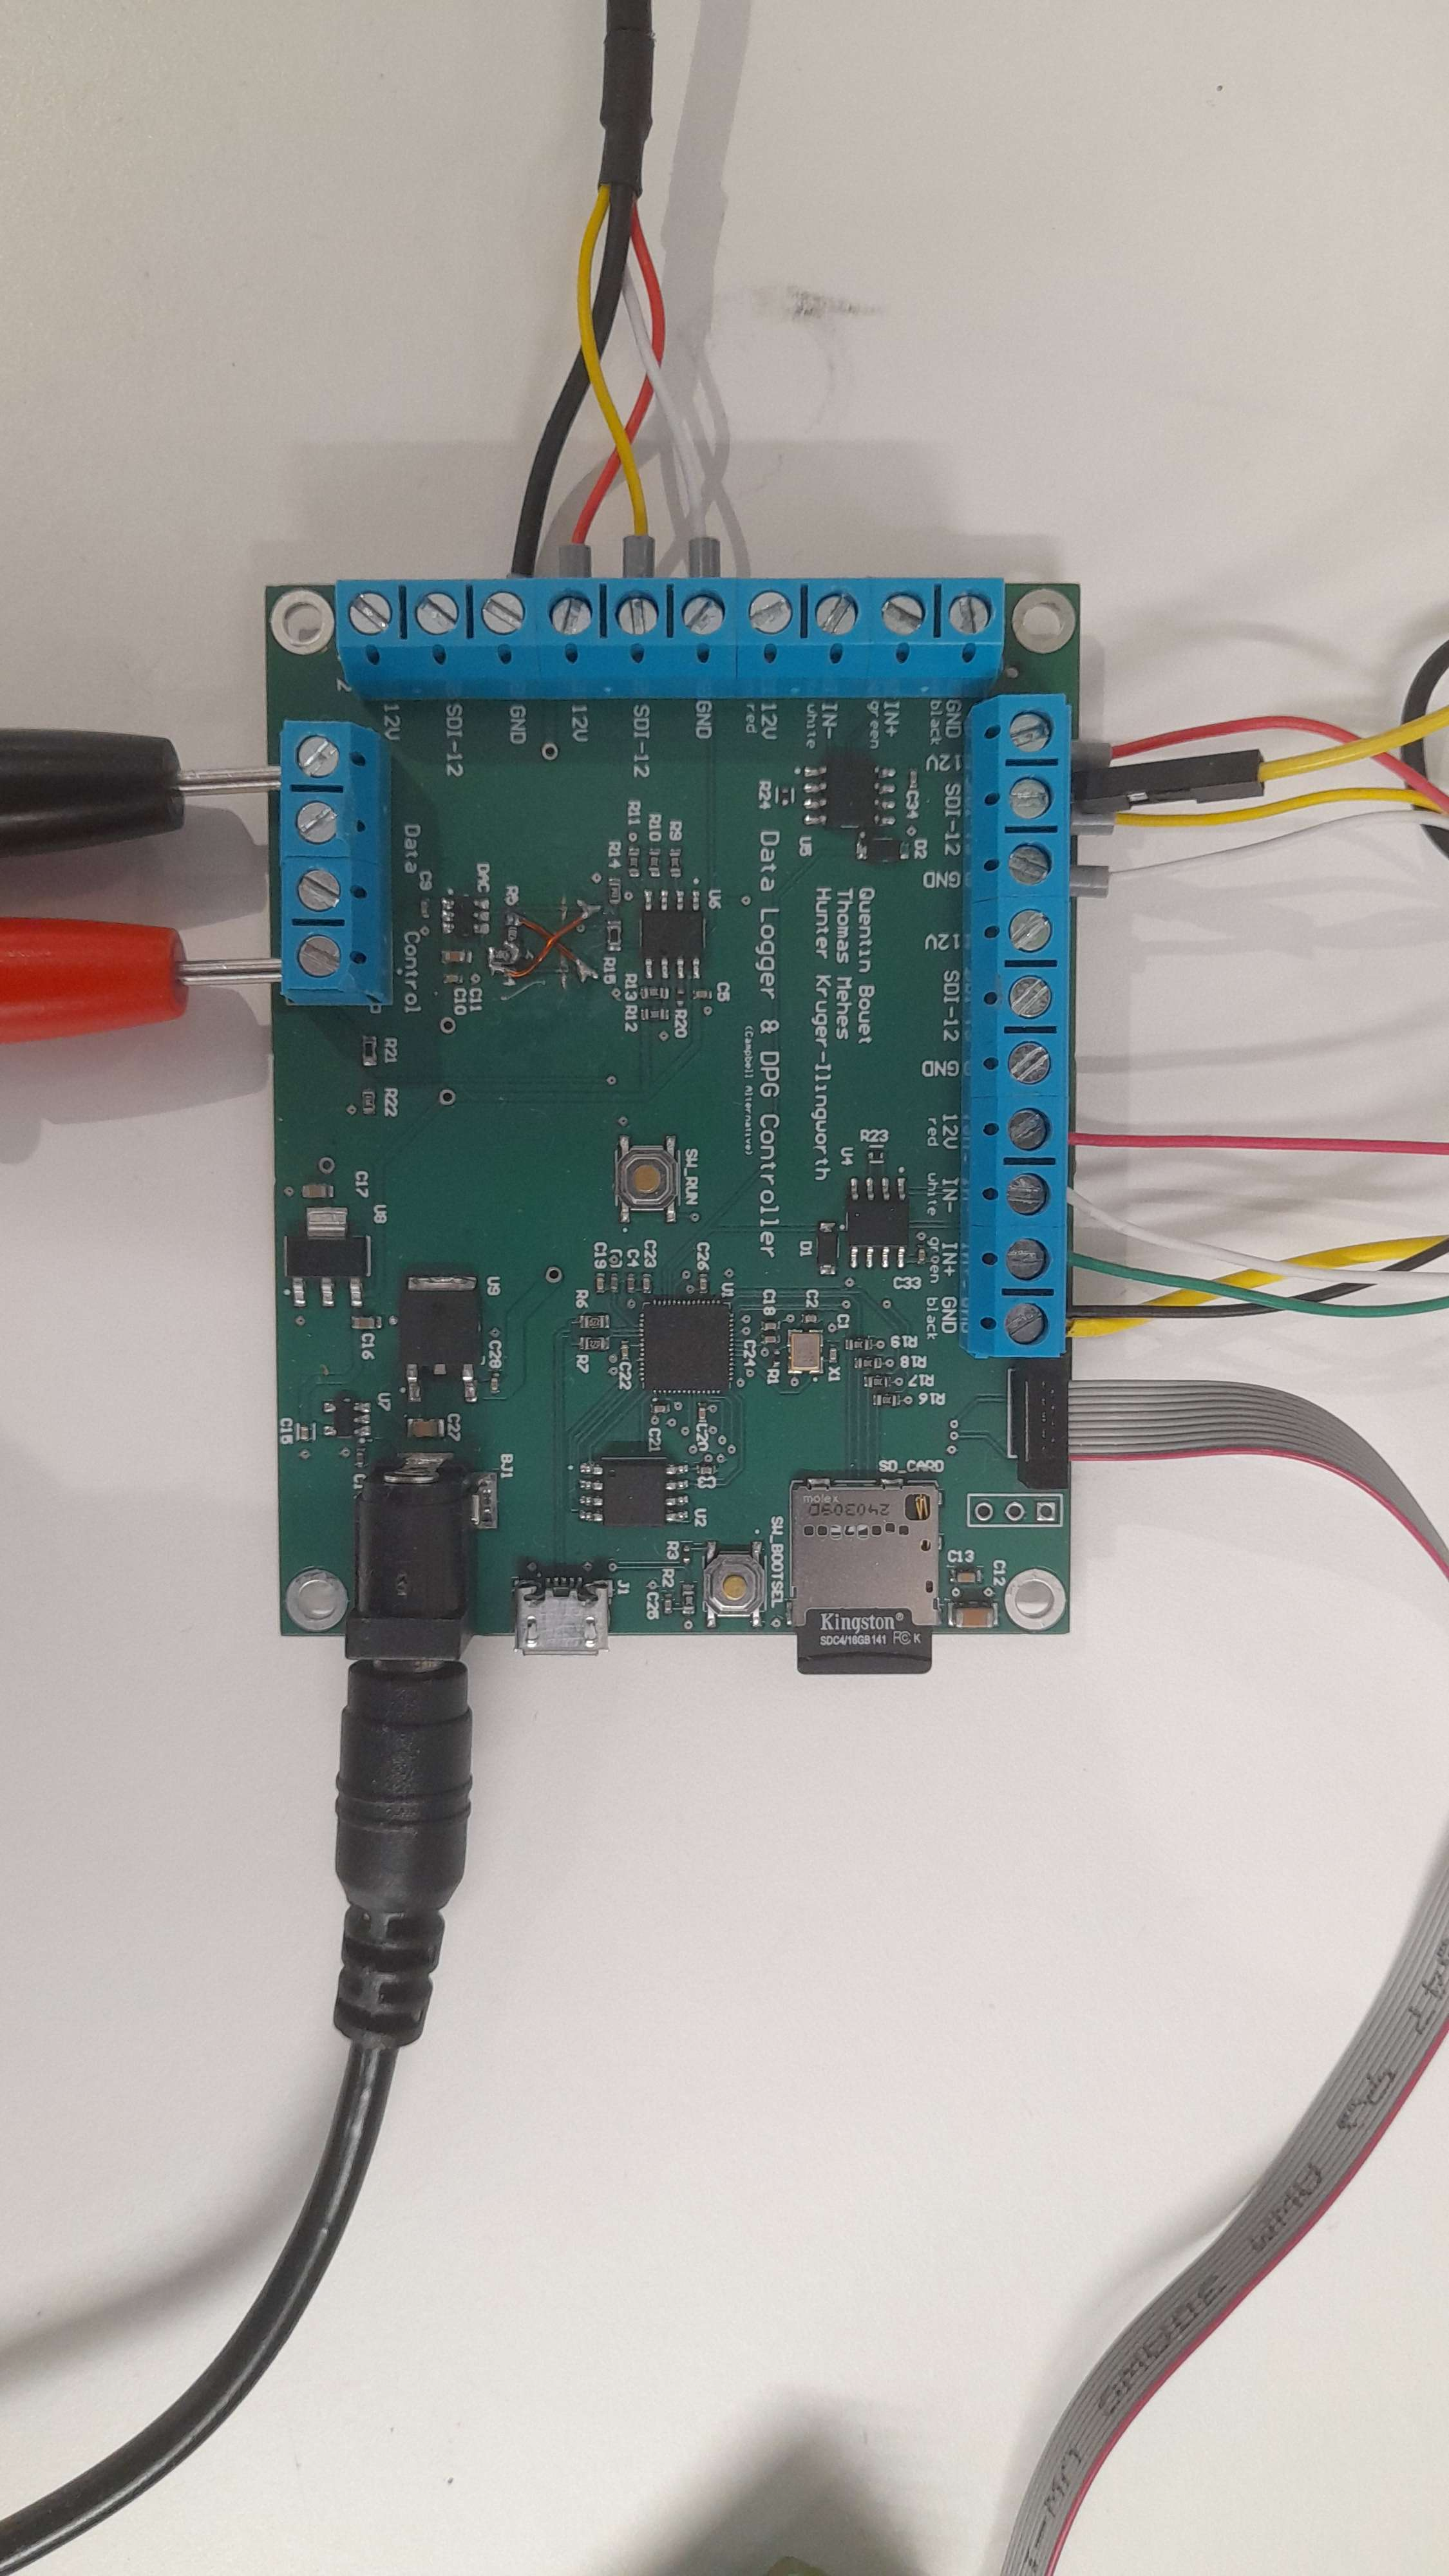
\includegraphics[width=\linewidth]{figures/board_photo.jpg}
    \caption{Photo of Board}
    \label{board_photo}
\end{figure}

\subsection{Hardware Design}

\subsubsection{Load Cell and ADC Integration}

The MT-603 load cell requires an ADC (Analogue-to-Digital Converter) for signal conversion, as its output is an analogue 
signal representing weight measurements. Therefore, one of the RP2040's ADC pins was utilised 
to convert the load cell's voltage output into a digital signal in which the microcontroller 
can process. An instrumentation amplifier was also added to amplify the small voltage changes 
from the load cell, improving the resolution and accuracy of the measurements. This ADC 
integration allowed for precise scaling and calibration of the load cell to achieve 
accurate data representation.

\subsubsection{SDI-12 Sensors and Communication Interface} 

The SDI-12 protocol was implemented because 
it is the standard communication protocol for the environmental sensors integrated into 
this system. However, SDI-12 differs from typical UART communication in that its bit 
values are inverted and requires strict timing. To address this, the project leveraged 
the RP2040's UART capabilities in conjunction with an RS485 transceiver. The RS485 
transceiver is suitable for this application due to its robust line-driving capabilities, 
noise immunity, and compatibility with inverted logic levels. By using only the non-inverting 
line of the differential pair (data line B), and setting the voltage reference at 2.5V, the design 
effectively maps the inverted SDI-12 signals to conventional UART high and low values, 
allowing reliable sensor communication.

\subsubsection{Power Supply and Voltage Regulation}

Due to the diversity of communication protocols 
and components used in the system (such as ADC for the load cell, SDI-12 for sensors, and I2C 
for the DAC—multiple), the following voltage levels were required on the PCB: 12V, 5V, and 3.3V. Each voltage 
level was supplied through dedicated regulators to ensure stable power delivery to each module. 
The careful placement of decoupling capacitors was critical to minimize voltage ripple and noise, 
ensuring stable operation of the entire system.

\subsubsection{Data Logging and Storage}

An SD card module was added to the schematic, utilising the 
SPI interface as defined in the RP2040 datasheet. This module enables reliable data storage 
and allows easy access to logged data for further analysis. The SPI bus operates at a clock 
speed of 1 MHz, which is suitable for reliable data transfer with the SD card.

\subsubsection{DAC Integration}

Initially, a solution consisting of Pulse Width Modulation (PWM) 
along with a low pass filter was considered to convert to generate the required analogue signal 
for the dew point generator. However, this method proved unreliable and inaccurate when tested 
with a Raspberry Pi Pico. As a result, the MCP4716 DAC (10 bits) was integrated to provide fine-grained control of 
the dew point generator. Proper bypass capacitors were placed near the $V_{DD}$ pin 
to minimize induced noise and ensure stable operation. The DAC was designed to communicate with the RP2040 
over the I2C bus at a standard mode speed of 100 kHz.